\section{Methodology}\label{sec:method}
%\david{Figure out how we want to present this clearly as we use a lot of `black boxes'}
%\david{We might want to rename this to utterance embeddings? And then hace a seperate section on the actual methodology?}
%
%\begin{itemize}
%	\item How do we find utterance embeddings?
%	\item Use these as features
%	\item For ML algorithms (NN, SVM, NB?, Nearest Neighbor)
%	\item maybe here something on datasets?
%	\item ...
%\end{itemize}

\subsection{Utterance embeddings} 

In order to get vector representations from utterances, we use an extension of the word embeddings neural network proposed by Mikolov\cite{mikolov2013efficient}. Originally, these networks had two main architectures, know as \emph{Continuous-bag-of-words} and \emph{Skip-gram}. In the first case, they were optimized so as to predict the next word given its context, while in the latter, a word is input and the context is predicted. Due to word co-occurrences, these models are able to effectively capture the meaning of the words. The co-occurrence property present at the word level is no longer valid when handling phrases. For sentence embeddings a novel approach was recently introduced \lau{cite}, in which a similar training algorithm is followed. In this case, two structures are maintained (one for words, and one for sentence representations); the word structure is shared across all sentences, while the sentence structure is only valid for the current paragraph. The task is the same as before: given a certain window, the model is optimized to predict the missing word; but this time, the context representation is constructed using the individual word vectors as well as the paragraph vector. This training schema is called \emph{Paragraph Vector Distributed memory (PV-DM)}, and it is the one we use to train our model. Figure~\ref{fig:p2v_arq} shows the \emph{PV-DM} architecture.

\begin{figure}
\centering
\begin{minipage}{.3\textwidth}
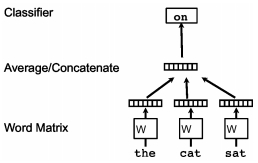
\includegraphics[width=1\textwidth]{img/par2vec_arq}
\caption{Paragraph vector PV-DM architecture.}
\label{fig:p2v_arq}
\end{minipage}
\end{figure}

Once the model is trained, it can be queried so as to get the vector representations for each already seen sentence. It can also be used to \emph{infer} vector mappings of \emph{unseen} sentences. This second step will be crucial to get representations for utterances in our test dataset.

A great advantage of these approach is that it is completely unsupervised, and thus, we can use any amount of unlabelled data we want.

\subsubsection*{Word2vec pretrained vectors}
The implementation we use for getting paragraph vectors allows us to use already trained word embeddings. The way in which this feature works follows can be summarized as: (a) No new words are added to the vocabulary; (b) Intersecting words adopt pretrained values ; (c) Non intersecting words are left alone.
For our experiments, we try both alternatives, training word and paragraph embeddings from scratch using several dialog corpora as input, and also using freely available embeddings\footnote{\url{https://code.google.com/p/word2vec/}}.

\subsection{Dialog datasets}
\lau{Describe the switchboard corpus. It's 42 tags.}
\lau{Describe the BNC corpus.}
Throughout the classification pipeline, we make use use different dialog corpora. With the purpose of training word embedding models, options include training using a combination of: the Switchboard corpus, the British National corpus, and pretrained word vectors.

For the evaluation step is mandatory to utilize labelled data, for this reason, we train and evaluate our classifiers on the Switchboard corpus. We divide the dataset into a training and a validation set, containing $\%$ and $\%$ of the total length, respectively. \lau{add percentages}

In the next subsections we present a description of each dataset.

\subsubsection*{The Switchboard corpus}
The Switchboard Dialog Act corpus (SwDA) consists of a compilation of telephone transcriptions between two participants. It contains a total 205.000 utterances and 1.4 million words
While many features are defined for each utterance unit, the most important for our work is the tag attribute. Each utterance is associated to a label, which summarizes syntactic, semantic, and pragmatic information. The corpus contains a total of 200 tags, which can be further aggregated into 44 main classes. Table~\ref{tab:swda_tag_example} shows examples for the five most common tags. Table~\ref{tab:swda_sent_example} present examples of utterances contained in the SwDA corpus.

\lau{add cite to SWDA}

\begin{table}[h]
\centering
\begin{tabular}{l l l c}
\hline
\textbf{Tag} & \textbf{Description} & \textbf{Example} & \textbf{\%}\\
\hline
st & Statement-non-opinion & Me, I'm in the & 36 \\
 & & legal department. & \\
b & Acknowledge & Acknowledge Uh-huh. & 19 \\
sv & Statement-opinion & I think it's great. & 13 \\
aa & Accept & That's exactly it. & 5 \\
\% & Turn exit & So,- & 5 \\
 \hline
\end{tabular}
\caption{SWDA's 5 most frequent tags.}
\label{tab:swda_tag_example}
\end{table}

\begin{table}[h]
\centering
\begin{tabular}{p{0.45\textwidth}}
\hline
qrr B.34.utt2: {C or } do you think that [ we're, + we're, ] {F uh, } all trying to keep up with a certain standard of living? \\
sv A.35.utt1: I think that's part of it too. \\
sv A.35.utt2: {C But } I do think, - \\
qy B.36.utt1: {E I mean } do you think, \\
\hline
\end{tabular}
\caption{SwDA utterance examples.}
\label{tab:swda_sent_example}
\end{table}

\subsubsection*{The British National corpus}
The British National corpus (BNC) is a collection of 100 million words sampled from different written and spoken sources, with the intention of representing the British English language. Some of the sources of these data include newspapers, articles, journals, books, letter, transcription of informal conversations, among others. This dataset contains a huge amount of unlabelled sentences.
Table~\ref{tab:bnc_sent_example} presents sentence examples extracted from the BNC.

\begin{table}[h]
\centering
\begin{tabular}{p{0.45\textwidth}}
\hline
ADR 172 The kind of girl that even if you didn't know well you always said "hello" to and got a cheery wave and a smile back. \\
B72 966 For example, the sedimentary rocks that form the top geological layer in much of southern Britain may be only a few hundred metres thick in a few isolated sites. \\
B2E 714 Then Fulham got one of her worst raids of the war. \\
 \hline
\end{tabular}
\caption{BNC sentence examples.}
\label{tab:bnc_sent_example}
\end{table}

\subsection{Classifiers}
\lau{Mention which classifiers we use, and with which params}